
\documentclass[11pt]{article}
\usepackage[utf8]{inputenc}
\usepackage[spanish]{babel}
\usepackage[margin=2.5cm]{geometry}
\usepackage{booktabs}
\usepackage{graphicx}
\usepackage{float}

\title{Informe de Calidad de Datos (DQR) \\ \large Proyecto AASIM -- Fase 2}
\author{Juan Manuel Buitrago \and Luis Carlos Rocha \and German Alberto Hidalgo}
\date{\today}

\begin{document}
\maketitle

\section*{Alcance de la muestra}
Este informe se elaboró sobre 30 sujetos y 1488 ventanas de PulseDB v2.0 (MIMIC-III y VitalDB), procesadas con la cadena de filtrado causal y la compuerta de calidad SQI del proyecto (\texttt{src/preprocessing/filters.py}, \texttt{src/sqi/quality\_assessment.py}).

\section{Compuerta de calidad SQI (RF4)}
\begin{itemize}
  \item Umbrales de aceptación: bSQI $\geq$ 0.85, kSQI $\geq$ 5.0, pSQI $\geq$ 0.50.
  \item Ventanas válidas (\texttt{quality\_flag == 0}): 45.09\%
  \item Etiquetas fuera de la censura hemodinámica (PAS 70--240, PAD 40--140, PP $\geq$ 20 mmHg, PAS $>$ PAD): 112 de 1488.
\end{itemize}

\begin{table}[H]
\centering
\begin{tabular}{lrrr}
\toprule
Criterio & Umbral & Ventanas rechazadas & Porcentaje (\%) \\
\midrule
bSQI & 0.85 & 6 & 0.40 \\
kSQI & 5.00 & 139 & 9.34 \\
pSQI & 0.50 & 801 & 53.83 \\
\bottomrule
\end{tabular}
\caption{Rechazo por criterio de la compuerta SQI (una ventana puede incumplir más de uno).}
\end{table}

\section{Estadística univariada (ventanas válidas por SQI)}
\begin{table}[H]
\centering
\begin{tabular}{lrrrrrr}
\toprule
statistic & SBP (mmHg) & DBP (mmHg) & PP (mmHg) & bSQI & kSQI & pSQI \\
\midrule
count & 671.00 & 671.00 & 671.00 & 671.00 & 671.00 & 671.00 \\
null\_count & 0.00 & 0.00 & 0.00 & 0.00 & 0.00 & 0.00 \\
mean & 113.77 & 56.20 & 57.57 & 1.00 & 13.61 & 0.56 \\
std & 21.87 & 11.87 & 14.00 & 0.01 & 5.67 & 0.05 \\
min & 74.26 & 35.48 & 33.56 & 0.94 & 5.04 & 0.50 \\
25\% & 97.61 & 48.92 & 46.92 & 1.00 & 8.83 & 0.52 \\
50\% & 107.26 & 55.25 & 55.89 & 1.00 & 12.94 & 0.55 \\
75\% & 136.33 & 60.76 & 68.51 & 1.00 & 18.85 & 0.61 \\
max & 162.91 & 86.51 & 87.13 & 1.00 & 30.55 & 0.69 \\
\bottomrule
\end{tabular}
\caption{Estadística descriptiva de SBP, DBP, presión de pulso y los índices SQI.}
\end{table}

\section{Estadística bivariada}
\begin{table}[H]
\centering
\begin{tabular}{lrr}
\toprule
corr(SBP,DBP) & corr(SBP,PP) & corr(DBP,PP) \\
\midrule
0.82 & 0.87 & 0.43 \\
\bottomrule
\end{tabular}
\caption{Correlación de Pearson entre SBP, DBP y presión de pulso.}
\end{table}

\section{Cuotas ISO 81060-2 (mínimo exigido: 5\,\% por rango)}
\begin{table}[H]
\centering
\begin{tabular}{lrr}
\toprule
Rango & Porcentaje (\%) & Estado (min. 5\%) \\
\midrule
PAS <= 90 mmHg & 9.54 & Cumple \\
PAS >= 160 mmHg & 0.45 & No cumple \\
PAD <= 60 mmHg & 71.83 & Cumple \\
PAD >= 100 mmHg & 0.00 & No cumple \\
\bottomrule
\end{tabular}
\caption{Cobertura de rangos extremos de presión exigidos por ANSI/AAMI/ISO 81060-2.}
\end{table}

\section{Retención por paciente}
\begin{table}[H]
\centering
\begin{tabular}{lr}
\toprule
statistic & \% ventanas válidas (SQI) por paciente \\
\midrule
count & 30.00 \\
null\_count & 0.00 \\
mean & 40.09 \\
std & 45.30 \\
min & 0.00 \\
25\% & 0.00 \\
50\% & 13.33 \\
75\% & 91.67 \\
max & 100.00 \\
\bottomrule
\end{tabular}
\caption{Distribución del porcentaje de ventanas válidas por SQI, por paciente.}
\end{table}

\section{Figuras}
\begin{figure}[H]
\centering
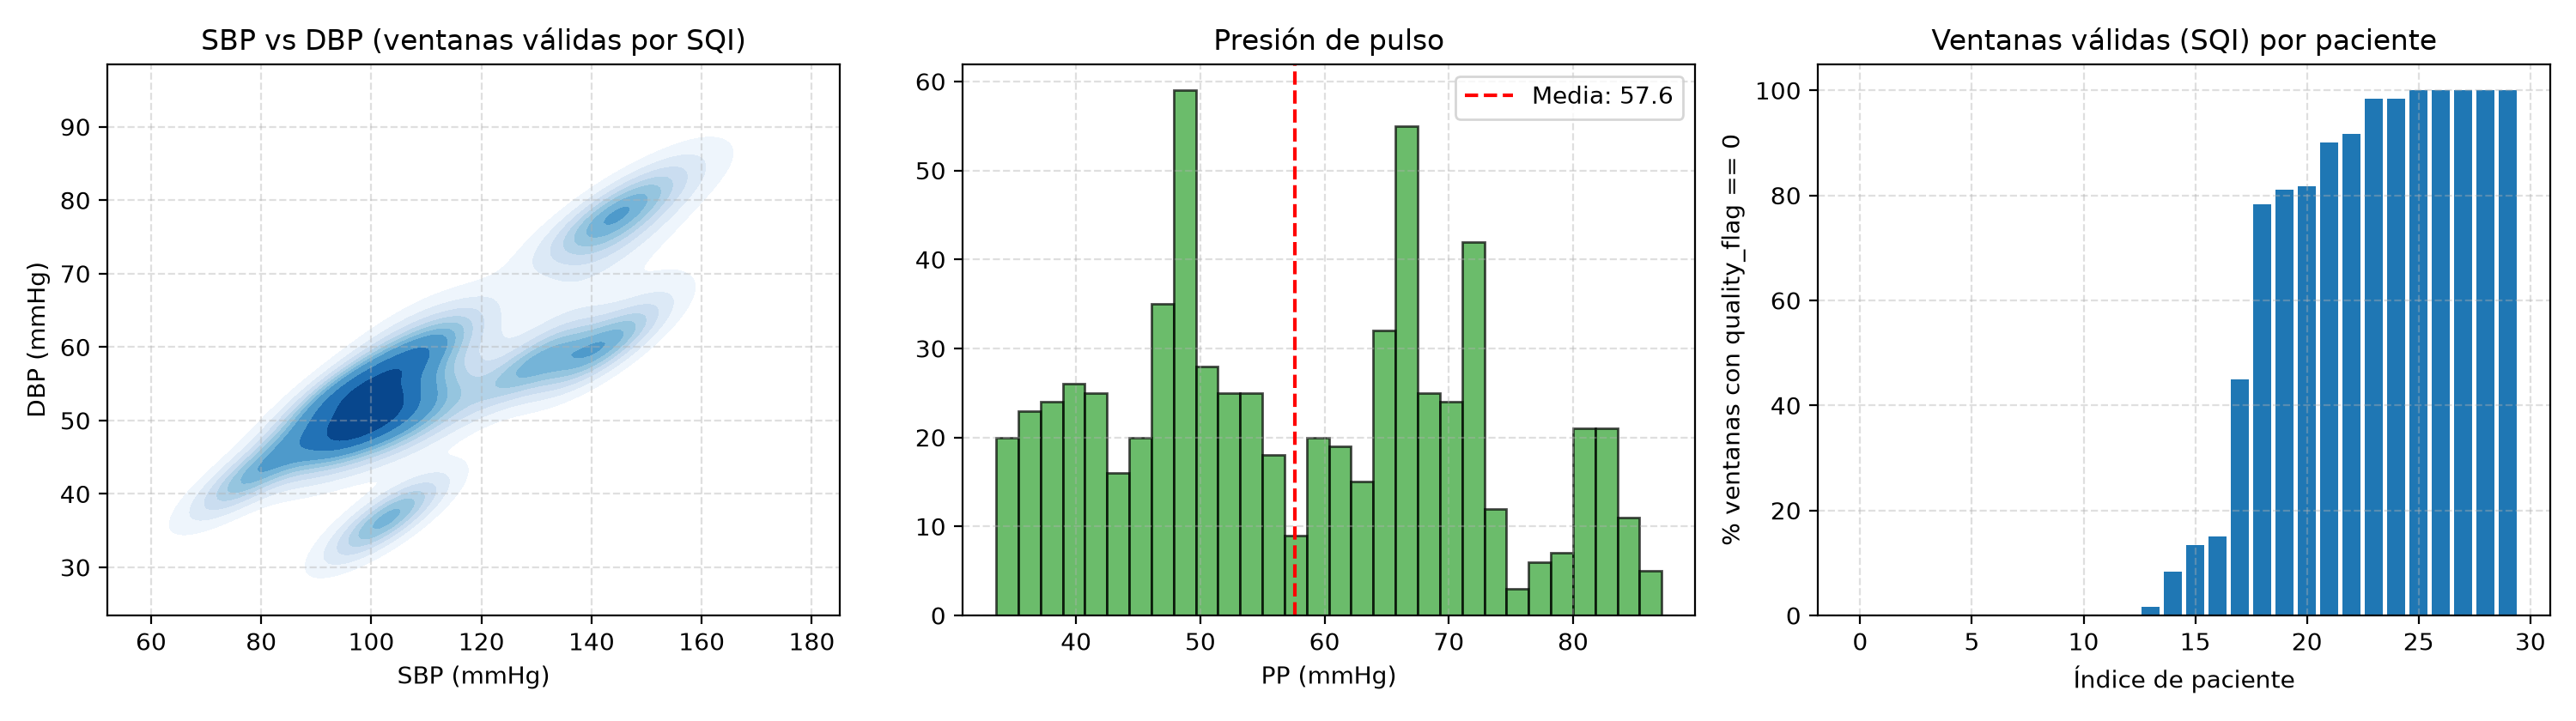
\includegraphics[width=\linewidth]{figuras/distribuciones.png}
\caption{Distribución conjunta SBP--DBP, presión de pulso y retención por paciente (compuerta SQI).}
\end{figure}

\end{document}
